\section{Портрет Чарльза Беббіджа}

Є портрет відомого англійського математика Чарльза Беббіджа
(рис. \ref{fig:practice:babbage}).
За допомогою бінарної функції витрат та дискретизації множини параметрів
було отримано навпрочуд реалістичну модель
(рис. \ref{fig:practice:babbage-model}).

\begin{figure}[h]
  \centering
  \begin{subfigure}[b]{0.4\textwidth}
    \centering
    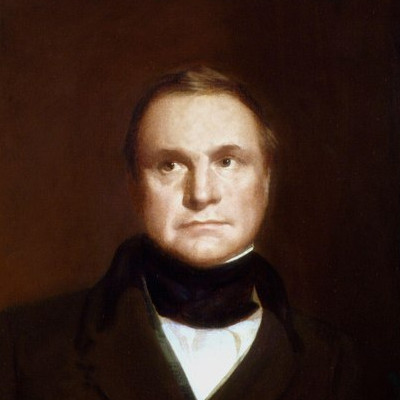
\includegraphics[width=\textwidth]{images/babbage}
    \caption{Фрагмент портрету}
    \label{fig:practice:babbage}
  \end{subfigure}
  \begin{subfigure}[b]{0.4\textwidth}
    \centering
    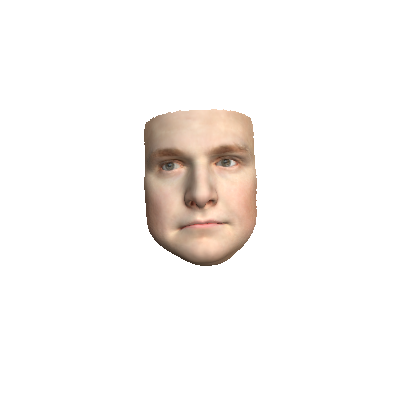
\includegraphics[width=\textwidth]{images/babbage-model}
    \caption{Реконструйована модель}
    \label{fig:practice:babbage-model}
  \end{subfigure}
  \caption{Чарльз Беббідж молодий}
\end{figure}

Проте реалістична текстура та тіні --- це не привід вважати,
що алгоритм відпрацював добре.
Тому було взято інший портрет вченого,
де він старше та дивиться в іншу сторону
(рис. \ref{fig:practice:babbage-old}).
До наявної моделі застосовано лише інший поворот та освітлення
(рис. \ref{fig:practice:babbage-model-rotated}),
ніякої додаткової інформації з портрету система не дістає.
Тепер можна оцінити якість реконструкції на око,
бо дійсної тривимірної моделі голови Беббіджа немає.

\begin{figure}[h]
  \centering
  \begin{subfigure}[b]{0.4\textwidth}
    \centering
    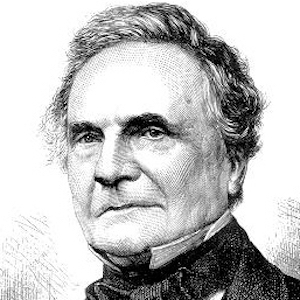
\includegraphics[width=\textwidth]{images/babbage-old}
    \caption{Портрет}
    \label{fig:practice:babbage-old}
  \end{subfigure}
  \begin{subfigure}[b]{0.4\textwidth}
    \centering
    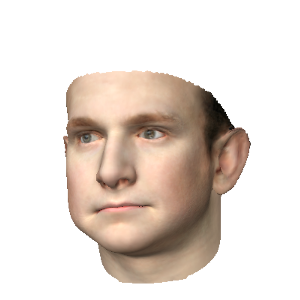
\includegraphics[width=\textwidth]{images/babbage-model-rotated}
    \caption{Повернена модель}
    \label{fig:practice:babbage-model-rotated}
  \end{subfigure}
  \caption{Чарльз Беббідж}
\end{figure}

З рисунку видно, що деякі ділянки реконструйовані некоректно.
Проте взагалом результат задовільний.
Отриману модель можна повернути під будь-яким кутом
(рис. \ref{fig:practice:babbage-profile})
та застосувати будь-яку тінь
(рис. \ref{fig:practice:babbage-shaded}).

\begin{figure}[h]
  \centering
  \begin{subfigure}[b]{0.3\textwidth}
    \centering
    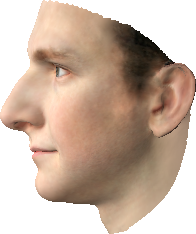
\includegraphics[width=\textwidth]{images/babbage-profile}
    \caption{Вигляд збоку}
    \label{fig:practice:babbage-profile}
  \end{subfigure}
  \begin{subfigure}[b]{0.3\textwidth}
    \centering
    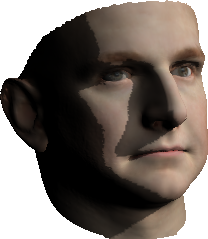
\includegraphics[width=\textwidth]{images/babbage-shaded}
    \caption{Інша тінь}
    \label{fig:practice:babbage-shaded}
  \end{subfigure}
  \caption{Реконструйована модель Чарльза Беббіджа}
\end{figure}
